\documentclass[aspectratio=169,11pt]{beamer}
\usetheme[progressbar=frametitle,numbering=fraction]{metropolis}
\usepackage{amsmath,amssymb,bm}
\usepackage{booktabs}
\usepackage{tikz}
\usetikzlibrary{arrows.meta,positioning,shapes.geometric}
\usepackage{listings}

% ---------------------------------------------------------------- colours
\definecolor{ink}{HTML}{2B2B2B}
\definecolor{muted}{HTML}{6B6B66}
\definecolor{cA}{HTML}{2A78D6}      % terms that go to A(y)
\definecolor{cB}{HTML}{14875E}      % terms that go to beta(y)
\definecolor{cP}{HTML}{D2541F}      % terms that go to phi(y) theta
\definecolor{soft}{HTML}{F4F3EF}
\setbeamercolor{normal text}{fg=ink}
\setbeamercolor{frametitle}{bg=ink,fg=white}
\setbeamercolor{progress bar}{fg=cP,bg=soft}
\setbeamercolor{alerted text}{fg=cP}
\setbeamercolor{block title}{bg=soft,fg=ink}
\setbeamercolor{block body}{bg=soft!50}
\newcommand{\cA}[1]{{\color{cA}#1}}
\newcommand{\cB}[1]{{\color{cB}#1}}
\newcommand{\cP}[1]{{\color{cP}#1}}
\newcommand{\mnote}[1]{{\small\color{muted}#1}}

\lstset{language=Matlab,basicstyle=\ttfamily\scriptsize,keywordstyle=\color{cA},
        commentstyle=\color{muted},columns=fullflexible,keepspaces=true,
        showstringspaces=false,frame=none,backgroundcolor=\color{soft}}

\title{Parameter Monitoring with Adaptive Observers}
\subtitle{Estimating T cells and patient-specific parameters in SARS-CoV-2}
\author{Juan E. Sereno}
\institute{Postdoctoral Researcher, University of Dubrovnik\\ Mini-course \,·\, Semana IE--IC 2026}
\date{26 October 2026}

\begin{document}

\maketitle

% =====================================================================
\begin{frame}{Today: a 4-step recipe}
\begin{enumerate}
  \setlength\itemsep{0.9em}
  \item \textbf{Model.} Write down the dynamics and decide what is \emph{measured}, what is \emph{unknown}.
  \item \textbf{Can we?} Observability (states) and identifiability (parameters).
  \item \textbf{Rewrite.} Put the model in the \alert{state-affine form}
        \[\dot x = A(y)\,x + \beta(y) + \varphi(y)\,\theta,\qquad y = Cx .\]
  \item \textbf{Design and code.} Copy the adaptive observer, check its assumptions, tune it, run it in MATLAB/Python.
\end{enumerate}
\vfill
\mnote{Two worked examples: \textbf{Ex.\,1} estimate $c_T$ \quad·\quad \textbf{Ex.\,2} estimate $c_T$ and $r$. \quad Both also recover the unmeasured T cells.}
\end{frame}

% =====================================================================
\begin{frame}{Why an adaptive observer?}
\centering
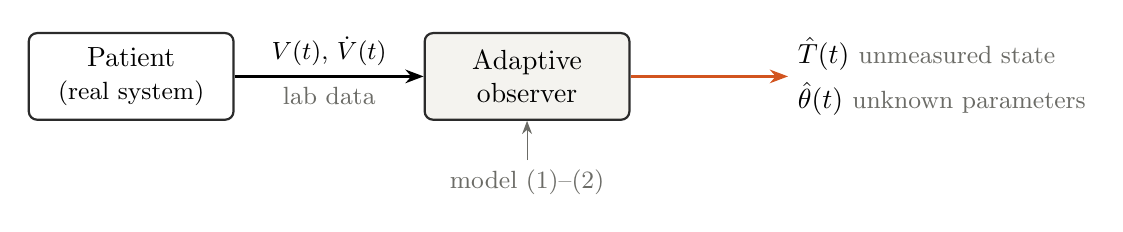
\begin{tikzpicture}[node distance=1.3cm,>=Stealth,
   box/.style={draw=ink,rounded corners=3pt,minimum height=1.1cm,minimum width=2.6cm,align=center,fill=white,thick}]
  \node[box] (P) {Patient\\ \small(real system)};
  \node[box,right=2.4cm of P,fill=soft] (O) {Adaptive\\ observer};
  \node[right=2.0cm of O,align=left] (E) {$\hat T(t)$ \mnote{unmeasured state}\\[3pt] $\hat\theta(t)$ \mnote{unknown parameters}};
  \draw[->,thick] (P) -- node[above]{\small $V(t)$, $\dot V(t)$} node[below]{\mnote{lab data}} (O);
  \draw[->,thick,cP] (O) -- (E);
  \node[below=0.5cm of O,align=center] (M) {\mnote{model (1)--(2)}};
  \draw[->,muted] (M) -- (O);
\end{tikzpicture}
\vspace{0.6cm}
\begin{itemize}
  \item We can measure the \textbf{viral load} $V$, but not the CD8$^+$ \textbf{T cells} $T$ that fight it.
  \item Parameters (killing rate, activation rate, \dots) are \textbf{different for every patient}.
  \item An adaptive observer estimates \textbf{states and parameters at the same time}, while data arrive: the basis of a \emph{digital twin}.
\end{itemize}
\end{frame}

% =====================================================================
\begin{frame}{Step 1 · The model (Hernandez-Vargas \& Velasco-Hernandez, 2020)}
\begin{columns}[T]
\begin{column}{0.52\textwidth}
\begin{align*}
\frac{dV}{dt} &= pV\Big(1-\frac{V}{K}\Big) - \alert{c_T}\,V\,T - cV \tag{1}\\[4pt]
\frac{dT}{dt} &= S_T + \alert{r}\,T\,\frac{V^m}{V^m+k_T^m} - \delta_T T \tag{2}
\end{align*}
\vspace{2pt}
\[ G(V) = \frac{V^m}{V^m+k_T^m}\quad \text{(T-cell activation)} \]
\[ \alpha = p-c,\qquad \sigma = p/K,\qquad \gamma = c_T S_T \]
\end{column}
\begin{column}{0.46\textwidth}
\footnotesize
\begin{tabular}{@{}lll@{}}
\toprule
 & meaning & ``mean'' patient\\
\midrule
$p$ & virus replication & 8.57 /day\\
$K$ & carrying capacity & $2.35\times10^{9}$\\
$c$ & virus clearance & 2.4 /day\\
\alert{$c_T$} & killing by T cells & $1.89\times10^{-6}$\\
\alert{$r$} & T-cell activation & 0.194 /day\\
$\delta_T$ & T-cell death & 0.1 /day\\
$k_T$, $m$ & half-sat., Hill & $1.26\times10^{5}$, 2\\
$S_T$ & replenishment $=\delta_T T_0$ & $10^{5}$\\
\bottomrule
\end{tabular}
\end{column}
\end{columns}
\end{frame}

% =====================================================================
\begin{frame}{Our virtual patient}
\centering
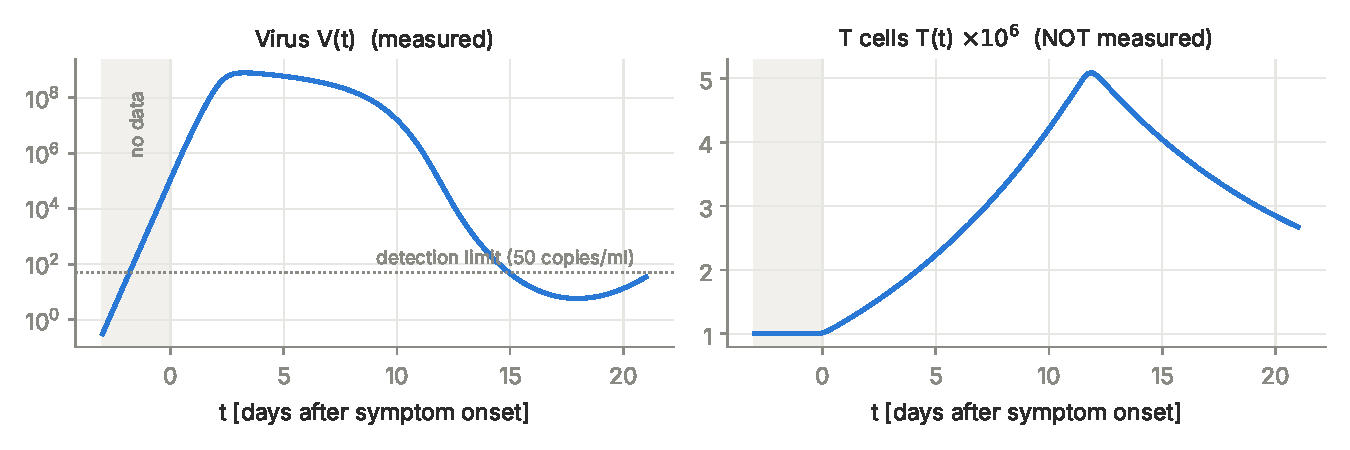
\includegraphics[width=0.92\textwidth]{figures/patient.pdf}
\begin{itemize}
  \item \textbf{Measured:} $V(t)$ (and its derivative $\dot V$) from $t=0$ (symptom onset).
  \item \textbf{Unknown:} $T(t)$ and the parameters $c_T$ (Ex.\,1) or $c_T, r$ (Ex.\,2).
\end{itemize}
\end{frame}

% =====================================================================
\begin{frame}{Step 2 · Can we do it?}
\begin{block}{Observability (Theorem 1 in the paper)}
With output $y=V$, stack $V$ and $\dot V$ and take the Jacobian w.r.t.\ $(V,T)$:
\[
\frac{\partial}{\partial(V,T)}\begin{bmatrix} V \\ \dot V\end{bmatrix}
=\begin{bmatrix} 1 & 0\\ \ast & -c_T V\end{bmatrix},
\qquad \det = -c_T V \neq 0 \iff V\neq 0 .
\]
$\Rightarrow$ T cells can be reconstructed \alert{as long as there is virus}.
\end{block}
\begin{block}{Identifiability (Theorem 2)}
The lumped parameters $\Theta=[\alpha,\sigma,\gamma,r,\delta_T]$ can be recovered from $V,\dot V,\ddot V,\dots$ ($\operatorname{rank}\partial\Phi/\partial\Theta = 5$).
\end{block}
\mnote{Rule of thumb: if these fail, no observer will work, however well you tune it.}
\end{frame}

% =====================================================================
\begin{frame}{Step 3a · A clever change of coordinates (Eq.\ 13)}
\[
x_1 = \frac{V}{\lambda},\qquad x_2 = \frac{\dot V}{\lambda}
\qquad\Longrightarrow\qquad y = \begin{bmatrix} y_1\\ y_2\end{bmatrix} = \underbrace{\begin{bmatrix} 1&0\\0&1\end{bmatrix}}_{C}\begin{bmatrix} x_1\\ x_2\end{bmatrix}
\]
\begin{itemize}
  \item Both new states are \textbf{measured} (assuming $\dot V$ is available).
  \item $T$ disappears from the equations. Solving (1) for it:
  \[
     \boxed{\;c_T\,T = \alpha - \sigma V - \frac{\dot V}{V}\;}
     \qquad\Rightarrow\qquad \hat T = \frac{\alpha-\sigma\hat V-\hat{\dot V}/\hat V}{\hat c_T}
  \]
  \item $\lambda = 10^8$ is only a \textbf{scaling} factor: $V$ reaches $10^9$, so we work with $x_1\sim 1$--$10$.
\end{itemize}
\end{frame}

% =====================================================================
\begin{frame}{The model in the new coordinates (Eq.\ 14)}
Differentiate $x_2$, replace $T$ and $\dot T$ using (1)--(2) \mnote{(see the handwritten derivation)}:
\begin{align*}
\dot x_1 &= x_2\\[3pt]
\dot x_2 &= \frac{x_2^2}{x_1} + (\alpha\delta_T - \alert{\gamma})\,x_1 - \lambda\delta_T\sigma\,x_1^2
            - \alert{r}\,\alpha\,x_1\,G + \lambda\,\alert{r}\,\sigma\,x_1^2\,G\\
         &\qquad - \delta_T\,x_2 - \lambda\sigma\,x_1x_2 + \alert{r}\,x_2\,G,
            \qquad G = G(\lambda x_1)
\end{align*}
\vspace{4pt}
\begin{itemize}
  \item Every term is a product of \textbf{known things}, \textbf{measured things} ($x_1=y_1$, $x_2=y_2$) and \alert{unknown parameters}.
  \item Nothing in it depends on $T$. That is why we changed coordinates.
\end{itemize}
\end{frame}

% =====================================================================
\begin{frame}{Step 3b · The state-affine form (Eq.\ 15): the recipe}
\[
\dot x = \cA{A(y)}\,x + \cB{\beta(y)} + \cP{\varphi(y)}\,\cP{\theta},\qquad y=Cx
\]
Sort every term of $\dot x$ into one of three bins:
\begin{enumerate}
  \setlength\itemsep{0.6em}
  \item \cP{\textbf{Contains an unknown parameter}} $\theta_i$ $\to$ column $i$ of $\cP{\varphi(y)}$.\\
        \mnote{The parameter must appear \emph{linearly}: $\theta_i\times(\text{function of } y)$.}
  \item \cA{\textbf{Known coefficient $\times\, x_j$}} $\to$ entry $(\cdot,j)$ of $\cA{A(y)}$.\\
        \mnote{Extra $x$'s become data: $\lambda\sigma x_1^2 = (\lambda\sigma\, y_1)\,x_1$.}
  \item \cB{\textbf{Only data and known constants}} $\to$ $\cB{\beta(y)}$.
\end{enumerate}
\vspace{4pt}
\begin{alertblock}{Golden rule}
$A$, $\beta$, $\varphi$ may only use \textbf{measured signals} $y$ and \textbf{known constants}, never $T$ and never $\theta$.
\end{alertblock}
\end{frame}

% =====================================================================
\begin{frame}{Example 1 · Unknown: $\theta = \gamma = c_T S_T$}
Regroup $\dot x_2$ (everything except $\gamma$ is known):
\[
\dot x_2 =
\underbrace{\cA{\big[\alpha(\delta_T - rG) + \lambda\sigma y_1(rG-\delta_T)\big]}}_{\cA{a_{21}(y)}}x_1
+\underbrace{\cA{\big[rG-\lambda\sigma y_1-\delta_T\big]}}_{\cA{a_{22}(y)}}x_2
+\underbrace{\cB{\frac{y_2^2}{y_1}}}_{\cB{\beta_2(y)}}
+\underbrace{\cP{(-y_1)}}_{\cP{\varphi_{2}(y)}}\cP{\gamma}
\]
\vspace{-2pt}
\[
\cA{A(y)}=\begin{bmatrix}0&1\\ a_{21}(y) & a_{22}(y)\end{bmatrix},\quad
\cB{\beta(y)}=\begin{bmatrix}0\\ y_2^2/y_1\end{bmatrix},\quad
\cP{\varphi(y)}=\begin{bmatrix}0\\ -y_1\end{bmatrix},\quad
C=I_2
\]
\begin{itemize}
  \small
  \item Why $\gamma$ and not $c_T$? $c_T\approx2\times10^{-6}$ but $\gamma\approx0.19$, and numbers of order 1 keep the solver happy. Then $\hat c_T = \hat\gamma/S_T$.
  \item \mnote{Freedom: $x_2^2/x_1$ could also go to $A$ as $(y_2/y_1)\,x_2$ (the paper's choice).}
\end{itemize}
\end{frame}

% =====================================================================
\begin{frame}{Example 2 · Unknowns: $\theta = [\gamma,\ r]^\top$}
Now $r$ is unknown too. Collect all the $r$-terms of (14) and factor out $r$:
\[
-r\alpha x_1G+\lambda r\sigma x_1^2G+r x_2G \;=\; \cP{r}\;\cP{G(y)\big(y_2-\alpha y_1+\lambda\sigma y_1^2\big)}
\]
\vspace{-4pt}
\[
\cA{A(y)}=\begin{bmatrix}0&1\\ \alpha\delta_T-\lambda\delta_T\sigma y_1 & -\delta_T-\lambda\sigma y_1\end{bmatrix},\qquad
\cB{\beta(y)}=\begin{bmatrix}0\\ y_2^2/y_1\end{bmatrix}
\]
\[
\cP{\varphi(y)}=\begin{bmatrix}0 & 0\\ -y_1 & G(\lambda y_1)\,\big(y_2-\alpha y_1+\lambda\sigma y_1^2\big)\end{bmatrix},\qquad
\cP{\theta}=\begin{bmatrix}\gamma\\ r\end{bmatrix}
\]
\begin{itemize}
  \item The $r$-terms \textbf{moved from $A$ to $\varphi$}. The observer equations do not change at all.
  \item \mnote{Physical meaning: $y_2-\alpha y_1+\lambda\sigma y_1^2 = -c_TVT/\lambda$ (killing by T cells).}
\end{itemize}
\end{frame}

% =====================================================================
\begin{frame}{Step 4 · The adaptive observer (Eq.\ 17)}
\begin{align*}
\dot{\hat x} &= A\hat x + \beta + \varphi\hat\theta + \big\{S^{-1}C^\top + \Lambda\Gamma^{-1}\Lambda^\top C^\top\big\}\,Q\,(y-C\hat x)
   && \text{\mnote{copy of the model + correction}}\\
\dot S &= -\rho_x S - A^\top S - SA + C^\top QC
   && \text{\mnote{state gain (Riccati-like)}}\\
\dot\Lambda &= \big(A - S^{-1}C^\top QC\big)\Lambda + \varphi
   && \text{\mnote{sensitivity } $\partial\hat x/\partial\hat\theta$}\\
\dot\Gamma &= -\rho_\theta\Gamma + \Lambda^\top C^\top QC\Lambda
   && \text{\mnote{accumulated information}}\\
\dot{\hat\theta} &= \Gamma^{-1}\Lambda^\top C^\top Q\,(y-C\hat x)
   && \text{\mnote{parameter update}}
\end{align*}
\vspace{2pt}
\begin{itemize}
  \item Sizes: $\hat x\in\mathbb R^{n}$, $S\in\mathbb R^{n\times n}$, $\Lambda\in\mathbb R^{n\times q}$, $\Gamma\in\mathbb R^{q\times q}$, $\hat\theta\in\mathbb R^{q}$. \quad Here $n=2$; $q=1$ (Ex.\,1) or $q=2$ (Ex.\,2).
  \item \textbf{Same five lines for any model} in state-affine form: only $A,\beta,\varphi,C$ change.
\end{itemize}
\end{frame}

% =====================================================================
\begin{frame}{How to read it}
\begin{itemize}
  \setlength\itemsep{0.7em}
  \item \textbf{Output error} $e = y - C\hat x$: the only signal that ``teaches'' the observer.
  \item $\bm\Lambda$ answers: \emph{``if $\hat\theta$ were a bit wrong, how would $\hat x$ move?''} It is driven by $\varphi$.
  \item $\bm\Gamma$ integrates $\Lambda^\top\Lambda$ with forgetting:
  \[
  \Gamma(t) = e^{-\rho_\theta t}\Gamma(0) + \int_0^t e^{-\rho_\theta(t-s)}\,\Lambda^\top C^\top QC\Lambda\,ds
  \]
  It measures \textbf{how much information we have collected} about $\theta$.
  \item $\dot{\hat\theta} = \Gamma^{-1}\Lambda^\top C^\top Q\,e$: a gradient step, scaled by the inverse of that information (like recursive least squares).
\end{itemize}
\end{frame}

% =====================================================================
\begin{frame}{Assumptions for convergence}
\small
\textbf{A1 · Uniform observability} of $\dot x = A(y)x,\ y=Cx$, with transition matrix $\Psi$:
\[\alpha_1 I\le\int_t^{t+T_1}\Psi^\top C^\top Q C\,\Psi\,ds\le\alpha_2 I\qquad\forall t\ge t_0\]
\textbf{A2 · Stable sensitivity:} with $L(t)=S^{-1}C^\top Q$ bounded,
\[\dot\Lambda = \big(A(y)-L(t)C\big)\Lambda \quad\text{is exponentially stable}\]
\textbf{A3 · Persistent excitation (PE)} of $\Lambda$, driven by $\varphi$ \;\mnote{(as in Eq.\,(4) of Aranovskiy et al.\ 2017)}:
\[\int_t^{t+T}\Lambda^\top C^\top Q C\,\Lambda\,ds\;\ge\;\mu\, I_q
  \quad\Longleftrightarrow\quad
  \lambda_{\min}\Big\{\int_t^{t+T}\Lambda^\top C^\top Q C\,\Lambda\,ds\Big\}\ge\mu>0
  \qquad\forall t\ge t_0\]
Also: $A$, $\beta$, $\varphi$ continuous and \textbf{bounded} along the trajectory.\\[4pt]
\mnote{If A1--A3 hold and $\rho_x,\rho_\theta$ are large enough, then $\hat x\to x$ and $\hat\theta\to\theta$ exponentially (Zhang 2002; Rodríguez et al.\ 2009, 2015).}
\end{frame}

% =====================================================================
\begin{frame}{The assumptions in plain words, for our examples}
\renewcommand{\arraystretch}{1.3}
\begin{tabular}{@{}p{0.2\textwidth}p{0.36\textwidth}p{0.38\textwidth}@{}}
\toprule
 & \textbf{Meaning} & \textbf{Our case}\\
\midrule
\textbf{A1} observability & from $y$ we can reconstruct $x$ & $C=I$: we measure all of $x$ \;\checkmark\\
\textbf{A2} stable $\Lambda$ & the correction $S^{-1}C^\top Q$ stabilises $A(y)$ & choose $\rho_x$ large (100) \;\checkmark\\
\textbf{A3} PE & the data must \emph{keep moving} so that $\theta$ shows its effect & $\varphi_{21}=-y_1\neq0$ only while the virus is high \alert{(days $\approx$\,2--10)}; see $\lambda_{\min}(\Gamma)$\\
bounded $A,\beta,\varphi$ & no division by zero & needs $V>0$: $y_2/y_1$, $y_2^2/y_1$ \alert{blow up if $V\to0$}\\
\bottomrule
\end{tabular}
\vspace{6pt}
\mnote{Lesson: \textbf{the observer can only learn while the infection is ``exciting'' the system.}}
\end{frame}

% =====================================================================
\begin{frame}{PE is a condition on the smallest eigenvalue}
\small
Compare with the gradient estimator for a linear regression $y=m^\top(t)\theta$ (Aranovskiy et al.\ 2017, Eq.\,4):
\[
\underbrace{\int_t^{t+T} m(s)\,m^\top(s)\,ds \;\ge\; \mu I_q}_{\text{regression}}
\qquad\longleftrightarrow\qquad
\underbrace{\int_t^{t+T} \Lambda^\top C^\top Q C\,\Lambda\,ds \;\ge\; \mu I_q}_{\text{our observer (A3)}}
\]
\begin{itemize}
  \setlength\itemsep{0.3em}
  \item $\Lambda$ plays the role of the regressor $m$: it is $\varphi$ \textbf{filtered} by the observer dynamics.
  \item ``$\ge\mu I$'' means \textbf{every eigenvalue} of the integral is $\ge\mu$, i.e.\ its \alert{minimal eigenvalue} is $\ge\mu$.
  \item Meaning: in every window of length $T$, the data push $\hat\theta$ in \textbf{every direction} of $\mathbb R^q$.
  \begin{itemize}
    \item Ex.\,1 ($q=1$): the integral is a scalar, $\int\Lambda^\top\Lambda\,ds>0$: $\Lambda$ must not stay at 0.
    \item Ex.\,2 ($q=2$): exciting $\gamma$ \emph{or} $r$ is not enough; the \textbf{least} excited direction decides.
  \end{itemize}
\end{itemize}
\end{frame}

% =====================================================================
\begin{frame}{An online PE meter: $\lambda_{\min}(\Gamma(t))$}
\small
$\Gamma(t)$ is the PE integral \textbf{with exponential forgetting}, and it is already inside the observer:
\[
\Gamma(t) = e^{-\rho_\theta t}\Gamma(0) + \int_0^t e^{-\rho_\theta(t-s)}\,\Lambda^\top C^\top QC\Lambda\,ds
\quad\Rightarrow\quad
\text{PE} \;\Longrightarrow\; \lambda_{\min}(\Gamma(t))\ge e^{-\rho_\theta T}\mu
\]
\vspace{-6pt}
\centering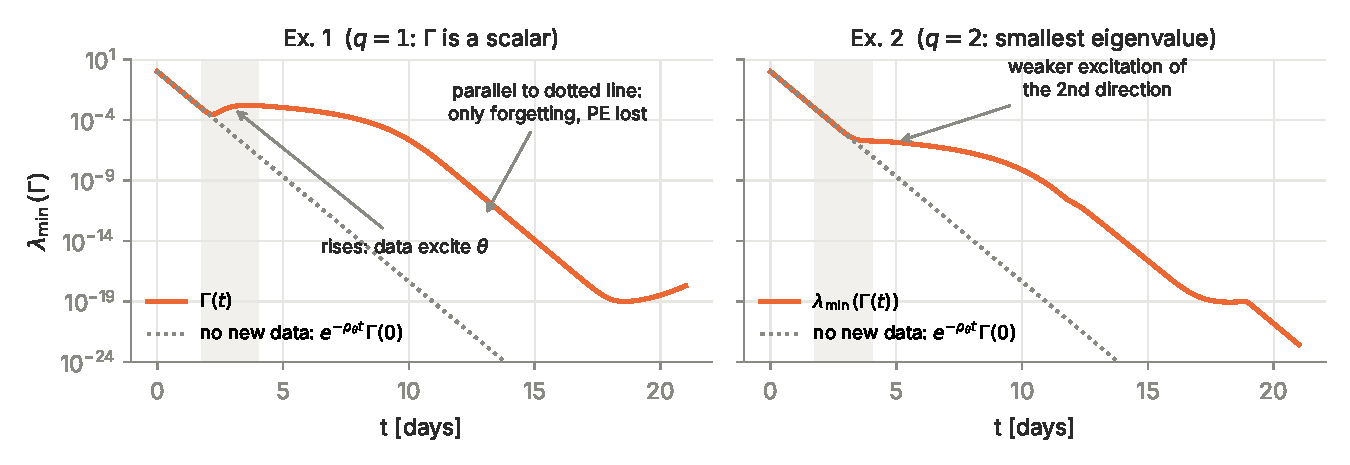
\includegraphics[width=0.82\textwidth]{figures/pe_meter.pdf}\\[-2pt]
\begin{itemize}
  \item Since $\dot{\hat\theta}=\Gamma^{-1}\Lambda^\top C^\top Q\,e$ and $\|\Gamma^{-1}\|=1/\lambda_{\min}(\Gamma)$: when PE is lost, the gain \alert{explodes} and noise drives $\hat\theta$.
\end{itemize}
\end{frame}

% =====================================================================
\begin{frame}{Tuning knobs}
\renewcommand{\arraystretch}{1.3}
\begin{tabular}{@{}lll@{}}
\toprule
Knob & Value used & Effect when you increase it\\
\midrule
$\rho_x$ & 100 & faster state correction, more sensitive to noise\\
$\rho_\theta$ & 4 & faster forgetting $\Rightarrow$ faster adaptation, noisier $\hat\theta$\\
$Q$ & $I_2$ & more weight on the output error\\
$\Gamma(0)$ & $I_q$ & larger $\Rightarrow$ smaller initial gain (slow start)\\
$S(0),\ \Lambda(0)$ & $I_2$, $0$ & usually not critical\\
$\hat x(0),\ \hat\theta(0)$ & $0.5\,y(0)$; $0.05$ & initial guesses (true: $\gamma=0.189$, $r=0.194$)\\
$\lambda$ & $10^8$ & scaling only: keeps $x_1$ of order 1--10\\
\bottomrule
\end{tabular}
\end{frame}

% =====================================================================
\begin{frame}[fragile]{From equations to code}
\begin{columns}[T]
\begin{column}{0.40\textwidth}
\small
One ODE for \textbf{patient + observer}. State vector (Ex.\,1, 11 entries):
\begin{tabular}{@{}ll@{}}
\texttt{z(1:2)} & $V,\ T$ \mnote{(patient)}\\
\texttt{z(3:4)} & $\hat x_1,\ \hat x_2$\\
\texttt{z(5:7)} & $S_{11},S_{12},S_{22}$\\
\texttt{z(8:9)} & $\Lambda$\\
\texttt{z(10)} & $\Gamma$\\
\texttt{z(11)} & $\hat\gamma$\\
\end{tabular}\\[6pt]
\mnote{Files: \texttt{Ex1\_main\_cT.m}, \texttt{Ex1\_AdapObs\_cT.m}, \texttt{patient\_model.m} \;(and \texttt{ex1\_cT.py})}
\end{column}
\begin{column}{0.58\textwidth}
\begin{lstlisting}
% measured data -> state-affine matrices
y1 = V/lambda;  y2 = dV/lambda;
A    = [0 1; a21 a22];
beta = [0; y2^2/y1];
phi  = [0; -y1];
C    = eye(2);

% adaptive observer, Eq. (17)
y_err  = y - C*x_hat;
dx_hat = A*x_hat + beta + phi*theta_hat ...
   + (S\C' + Lambda*(Gamma\Lambda')*C')*Q*y_err;
dS      = -rho_x*S - A'*S - S*A + C'*Q*C;
dLambda = (A - S\C'*Q*C)*Lambda + phi;
dGamma  = -rho_theta*Gamma + Lambda'*C'*Q*C*Lambda;
dtheta_hat = Gamma\Lambda'*C'*Q*y_err;
\end{lstlisting}
\end{column}
\end{columns}
\end{frame}

% =====================================================================
\begin{frame}{Results · Example 1 (estimate $c_T$)}
\begin{columns}[c]
\begin{column}{0.56\textwidth}
\centering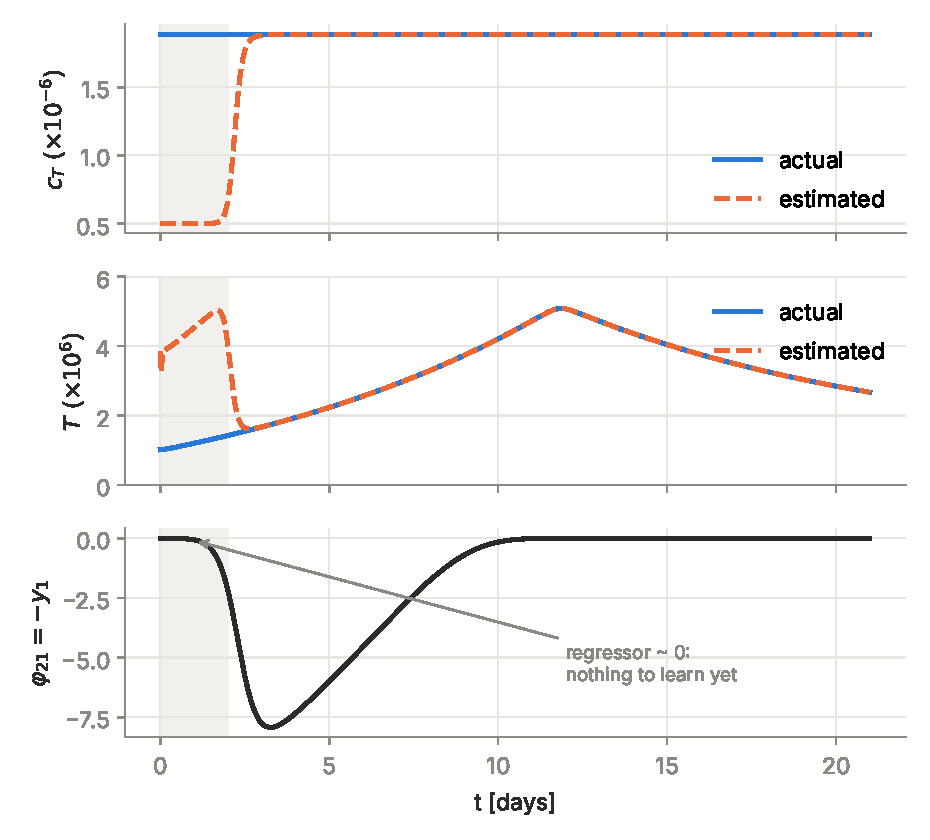
\includegraphics[height=0.78\textheight]{figures/ex1.pdf}
\end{column}
\begin{column}{0.42\textwidth}
\begin{itemize}
  \setlength\itemsep{0.8em}
  \item $\hat c_T$ reaches the true value by \textbf{day $\approx$ 4}.
  \item $\hat T$ is wrong while $\hat c_T$ is wrong, then follows $T$.
  \item \textbf{Shaded:} the first two days, when $\varphi_{21}=-y_1\approx0$. There is no excitation, so $\hat c_T$ \alert{cannot move} (A3).
\end{itemize}
\end{column}
\end{columns}
\end{frame}

% =====================================================================
\begin{frame}{Results · Example 2 (estimate $c_T$ and $r$)}
\begin{columns}[c]
\begin{column}{0.56\textwidth}
\centering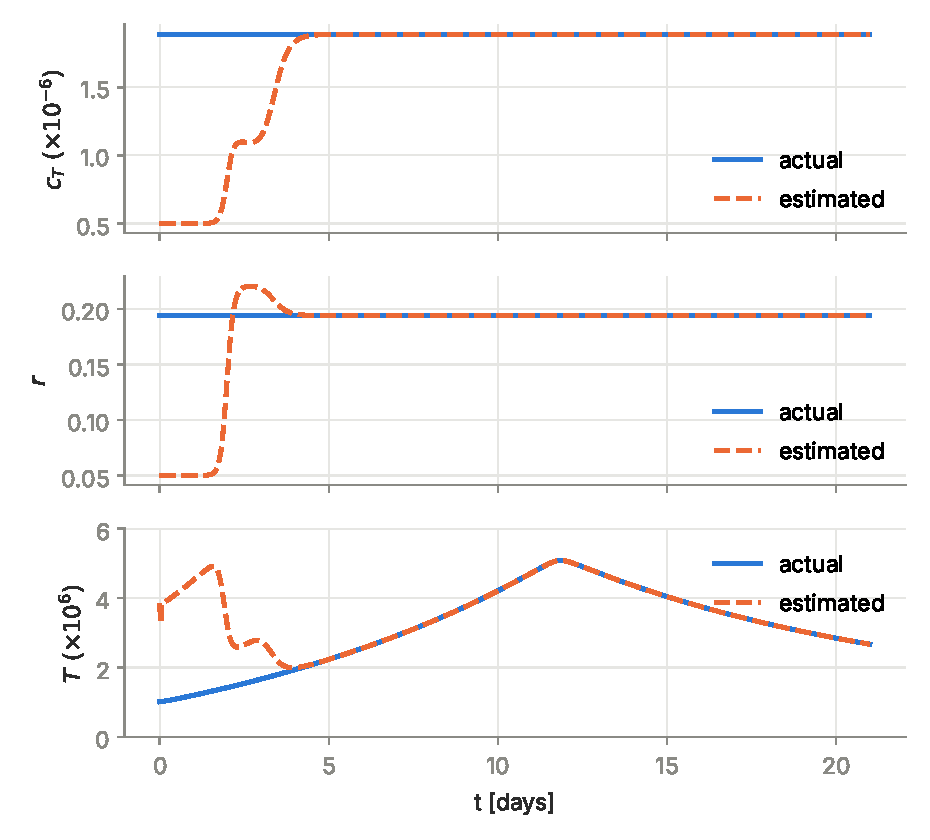
\includegraphics[height=0.78\textheight]{figures/ex2.pdf}
\end{column}
\begin{column}{0.42\textwidth}
\begin{itemize}
  \setlength\itemsep{0.8em}
  \item Both parameters converge by \textbf{day $\approx$ 6}.
  \item One more unknown means you \alert{need more excitation}, so convergence is slower (as in Table I of the paper).
  \item Same code: only $A$, $\varphi$ and the sizes of $\Lambda,\Gamma,\hat\theta$ changed.
\end{itemize}
\end{column}
\end{columns}
\end{frame}

% =====================================================================
\begin{frame}{With real data: noise, sampling, detection limits}
\centering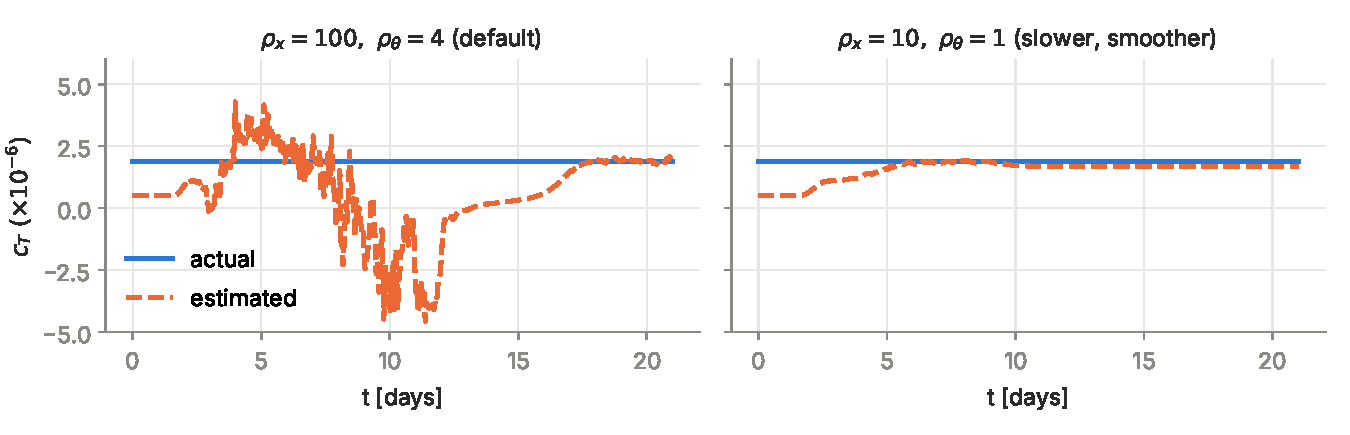
\includegraphics[width=0.74\textwidth]{figures/noise.pdf}\\[-4pt]
\mnote{Example 2, 5\% multiplicative noise on $V$. Left: default tuning. Right: smaller $\rho_x,\rho_\theta$ (more memory).}
\begin{itemize}
  \small
  \item \textbf{Noise:} the drift (days 7--12) appears when $\lambda_{\min}(\Gamma)$ is tiny. Trade speed for robustness with $\rho_x$, $\rho_\theta$.
  \item \textbf{$\dot V$ is not measured} in the clinic; it has to be estimated with numerical differentiators.
  \item \textbf{Detection limit:} below 50 copies/ml, $V\approx0$, so the $1/y_1$ terms and PE are both lost: stop adapting.
\end{itemize}
\end{frame}

% =====================================================================
\begin{frame}{Hands-on exercises}
\begin{enumerate}
  \setlength\itemsep{0.55em}
  \item \textbf{Run} Ex.\,1 and Ex.\,2. Change the initial guesses $\hat\theta(0)$ and $\Gamma(0)$. What changes?
  \item \textbf{Other patients:} use the parameter sets A--I of Hernandez-Vargas (2020). Which ones converge slowest, and why? \mnote{(Hint: look at $\varphi$.)}
  \item \textbf{Noise:} set \texttt{add\_noise = true}. Re-tune $\rho_x$ and $\rho_\theta$.
  \item \textbf{Start late:} start the observer at day 12. Is there still PE? Look at the PE meter $\lambda_{\min}(\Gamma(t))$.
  \item \textbf{Your turn:} estimate $\theta=[\gamma,\ \delta_T]$ instead. Find $A$, $\beta$, $\varphi$.\\
        \mnote{Hint: the $\delta_T$-column of $\varphi$ is $\alpha y_1-\lambda\sigma y_1^2-y_2$.}
\end{enumerate}
\end{frame}

% =====================================================================
\begin{frame}{Take-home recipe}
\begin{enumerate}
  \setlength\itemsep{0.8em}
  \item \textbf{Model}: what is measured ($y$), what is unknown ($x$, $\theta$)?
  \item \textbf{Check} observability and identifiability.
  \item \textbf{Change coordinates} so the unknown states disappear and the parameters enter \emph{linearly}.
  \item \textbf{Sort terms} into $\cA{A(y)}$, $\cB{\beta(y)}$, $\cP{\varphi(y)\theta}$, using only measured data.
  \item \textbf{Copy Eq.\,(17)}, check A1--A3 (above all, \alert{persistent excitation}), tune $\rho_x$, $\rho_\theta$.
\end{enumerate}
\vfill
\centering{\Large Thank you!}\\[2pt]
\mnote{Code (MATLAB \& Python) in the course folder.}
\end{frame}

% =====================================================================
\begin{frame}{References}
\scriptsize
\begin{itemize}
  \setlength\itemsep{0.15em}
  \item A.~Rodríguez-Liñán, J.~E.~Sereno, G.~Quiroz-Compean, E.~A.~Hernandez-Vargas. \emph{Adaptive observers for calibrating immune digital twins in viral infections.} IEEE CDC, 2025.
  \item E.~A.~Hernandez-Vargas, J.~X.~Velasco-Hernandez. \emph{In-host mathematical modelling of COVID-19 in humans.} Annual Reviews in Control 50:448--456, 2020.
  \item Q.~Zhang. \emph{Adaptive observer for MIMO linear time-varying systems.} IEEE TAC 47(3):525--529, 2002.
  \item A.~Rodríguez, J.~De León, R.~Femat, C.~Hernández-Rosales. \emph{A dynamic parameter estimator to control chaos with distinct feedback schemes.} CNSNS 14(12):4280--4291, 2009.
  \item A.~Rodríguez, G.~Quiroz, R.~Femat, H.~Méndez-Acosta, J.~de León. \emph{An adaptive observer for operation monitoring of anaerobic digestion wastewater treatment.} Chem.\ Eng.\ J.\ 269:186--193, 2015.
  \item J.~de León Morales, A.~Chaillet, A.~Loría, G.~Besançon. \emph{Output feedback control via adaptive observers with persistency of excitation.} IFAC 2005.
  \item S.~Aranovskiy et al. \emph{Performance enhancement of parameter estimators via dynamic regressor extension and mixing.} IEEE TAC, 2017.
  \item R.~Visentin, C.~Dalla Man, Y.~C.~Kudva, A.~Basu, C.~Cobelli. \emph{Circadian variability of insulin sensitivity: physiological input for in silico artificial pancreas.} Diabetes Technol.\ Ther.\ 17(1):1--7, 2015.
  \item C.~Ramírez Mazo, L.~Gómez-Echavarría, L.~Lema-Pérez, S.~Röblitz. \emph{A physiologically based mathematical model describing estradiol and progesterone actions on glucose-insulin dynamics throughout the menstrual cycle.} J.\ Theor.\ Biol.\ 631:112518, 2026.
\end{itemize}
\end{frame}

% =====================================================================
\begin{frame}{Open projects: PAE · undergrad thesis · master thesis}
\footnotesize
\begin{columns}[T]
\begin{column}{0.49\textwidth}
\begin{block}{1 · Circadian insulin sensitivity in T1D}\scriptsize
\textbf{Objective.} Design an adaptive observer that tracks the time-varying insulin sensitivity $S_I(t)$ of a person with T1D from CGM and insulin-pump data, as in the breakfast/lunch/dinner pattern of Fig.\,1 in Visentin et al.\ (2015).\\[4pt]
\textbf{Methodology.}\vspace{-4pt}
\begin{enumerate}\setlength\itemsep{1pt}\setlength\topsep{1pt}
  \item Glucose--insulin minimal model with $S_I$ as unknown parameter.
  \item Rewrite it in state-affine form; check observability, identifiability and PE (meals as excitation).
  \item Generate in silico data with a circadian $S_I$ profile.
  \item Tune $\rho_\theta$ to follow $S_I$ changes; test noise and 5-min CGM sampling.
\end{enumerate}
\end{block}
\end{column}
\begin{column}{0.49\textwidth}
\begin{block}{2 · Menstrual cycle and diabetes}\scriptsize
\textbf{Objective.} Estimate the cycle-dependent insulin sensitivity $S_I(E_2,P_4)$ along the menstrual cycle of women with diabetes, based on the model of Ramírez Mazo et al.\ (2026).\\[4pt]
\textbf{Methodology.}\vspace{-4pt}
\begin{enumerate}\setlength\itemsep{1pt}\setlength\topsep{1pt}
  \item Adapt the $G$--$I$ part of the model to diabetes (exogenous insulin input).
  \item Choose the unknown parameters of $S_I(E_2,P_4)$ and write the state-affine form.
  \item Analyse observability, identifiability and PE over a 28-day cycle.
  \item Validate the observer in silico with $E_2$, $P_4$ profiles and CGM data.
\end{enumerate}
\end{block}
\end{column}
\end{columns}
\end{frame}

\end{document}
